\documentclass[10pt,twocolumn]{article}

% --- Page geometry: tight for 3 pages ---
\usepackage[
  letterpaper,
  top=0.65in, bottom=0.65in, left=0.6in, right=0.6in,
  columnsep=0.25in
]{geometry}

% --- Packages ---
\usepackage[T1]{fontenc}
\usepackage{times}              % compact serif font
\usepackage{microtype}          % better spacing
\usepackage{graphicx}
\usepackage{booktabs}
\usepackage{tabularx}
\usepackage{xcolor}
\usepackage{tikz}
\usetikzlibrary{arrows.meta, positioning, calc, shapes.geometric, fit}
\usepackage{caption}
\usepackage[colorlinks,citecolor=blue!70!black,urlcolor=blue!70!black,linkcolor=black]{hyperref}
\usepackage{enumitem}
\setlist{nosep, leftmargin=1.2em}
\usepackage{titlesec}
\usepackage{float}
\usepackage{balance}

% --- Compact sections ---
\titleformat{\section}{\bfseries\normalsize}{\thesection.}{0.4em}{}
\titlespacing*{\section}{0pt}{6pt plus 2pt}{2pt plus 1pt}
\titleformat{\subsection}{\bfseries\small}{\thesubsection}{0.4em}{}
\titlespacing*{\subsection}{0pt}{4pt plus 2pt}{1pt plus 1pt}
\titleformat{\subsubsection}[runin]{\bfseries\small}{}{0em}{}[.]
\titlespacing*{\subsubsection}{0pt}{3pt}{0.4em}

% --- Compact title ---
\makeatletter
\renewcommand{\maketitle}{%
  \twocolumn[%
    \begin{center}
      {\Large\bfseries \@title \par}
      \vskip 4pt
      {\normalsize \@author \par}
      \vskip 8pt
    \end{center}
  ]%
}
\makeatother

% --- Compact captions ---
\captionsetup{font=small, labelfont=bf, skip=4pt, belowskip=-4pt}

% --- Colors for figure ---
\definecolor{tiergreen}{HTML}{2E7D32}
\definecolor{tieramber}{HTML}{E65100}
\definecolor{tierred}{HTML}{C62828}
\definecolor{tierblue}{HTML}{1565C0}

% --- Footnote size reduction ---
\renewcommand{\footnotesize}{\fontsize{7.5pt}{9pt}\selectfont}

\begin{document}

\title{ClinFuse: Patient Entity Resolution\\Powered by MedGemma Clinical Reasoning}
\author{Alexander Rider}
\date{}
\maketitle

% =====================================================================
%  1  PROBLEM STATEMENT
% =====================================================================
\section{Problem Statement}

A cardiac arrest patient's duplicate record carried someone else's do-not-resuscitate order. The care team withheld life-saving treatment~\cite{ecri2016}. That case is far from unique: patients with duplicate charts are five times more likely to die during hospitalization~\cite{western2026}. Across 7{,}613 wrong-patient events at 181 healthcare organizations, 9\% resulted in patient harm~\cite{ecri2016}. For the emergency department registrar matching an unconscious patient to their records, or the IT staff reconciling patient feeds from dozens of hospitals, these are not edge cases---they are daily realities.

The scale of the problem matches its severity. An estimated 8--12\% of hospital records are duplicates~\cite{morris2016}, costing the U.S.\ healthcare system \$6.7 billion annually~\cite{blackbook2018}. Match accuracy averages 80--90\% within institutions but falls to 50\% in cross-organizational exchange~\cite{onc2014}---meaning roughly half of cross-organizational duplicates go unresolved. The MATCH~IT Act (H.R.~2002, 2025) sets a 99.9\% matching target~\cite{matchit2025}, and TEFCA v2.1 makes cross-organizational matching critical national infrastructure~\cite{tefca2024}. Closing this gap would resolve 99.8\% of currently-missed cross-organizational duplicates (from 50\% unresolved to 0.1\%). Even conservatively attributing half of the \$6.7B burden to cross-organizational failures, this represents over \$3~billion in recoverable annual waste---alongside the patient harm that fragmented records cause.

The barrier isn't better algorithms---it's better information. Any method relying exclusively on demographic fields faces an accuracy ceiling imposed by field quality---over half of duplicate pairs contain misspelled names or mismatched identifiers~\cite{morris2016}. The missing signal is \emph{clinical context}: two records sharing the same disease trajectory, medication regimen, and vital sign patterns are almost certainly the same patient, regardless of demographic discrepancies---but interpreting clinical histories as identity evidence requires medical reasoning that traditional matching systems cannot perform.

% =====================================================================
%  2  OVERALL SOLUTION
% =====================================================================
\section{Overall Solution}

To demonstrate MedGemma's potential for patient entity resolution, we embed it in ClinFuse, a three-tier pipeline that augments fast probabilistic matching with MedGemma's clinical reasoning, invoked selectively for ambiguous cases. Figure~\ref{fig:architecture} illustrates the architecture.

\subsubsection{Tier~1: Probabilistic Screening} All records enter Splink~v4~\cite{splink} for Fellegi--Sunter~\cite{fellegi1969} probabilistic linkage using expectation-maximization on demographic fields with Jaro--Winkler string similarity and term-frequency adjustment. Pairs with high match probability are auto-matched; pairs with very low probability are auto-rejected.

\subsubsection{Tier~2: Clinical LLM Classification} Ambiguous ``gray zone'' pairs---those where demographics alone are inconclusive---receive structured clinical summaries and are classified by a fine-tuned MedGemma~4B model, whose medical pretraining enables it to interpret clinical histories as identity evidence. Each patient's clinical history is summarized into a compact format: conditions grouped by onset year, medications with date ranges, sorted allergies, latest values per vital sign, and procedures with years. The model sees two parallel summaries and classifies whether they describe the same patient (Figure~\ref{fig:example}).

\subsubsection{Tier~3: Score Fusion} The probabilistic match score and the LLM's classification logit are combined in log-odds space using interpretable linear weights. A demographic veto floor prevents the LLM from overriding cases where demographics strongly disagree, guarding against false merges---the highest-risk failure mode in clinical settings. This interpretable design ensures each component's contribution is transparent and auditable.

\subsubsection{Golden Records} Matched pairs form a graph whose connected components yield patient clusters. Field-level conflict resolution applies majority voting with domain heuristics (e.g., preferring longer address forms), producing a deduplicated Master Patient Index (MPI).

\smallskip
\noindent\textbf{MedGemma as Clinical Reasoner.}
Prior work has applied LLMs to adjacent healthcare tasks---MedLink uses
diagnosis-code embeddings for de-identified record
linkage~\cite{medlink2023}, and PRISM fine-tunes an LLM for clinical trial
matching~\cite{prism2024}---but neither addresses patient-to-patient identity
resolution using clinical narratives. In general-domain entity resolution,
large language models such as GPT-4 achieve strong zero-shot matching that
rivals fine-tuned pre-trained language models~\cite{peeters2023}, and
cost-efficient frameworks selectively route only uncertain pairs to an
LLM~\cite{booster2024,coling2025}---an architecture ClinFuse shares. However,
these approaches rely on cloud-hosted models with 70B--175B+ parameters,
incurring per-query costs, introducing latency, and---critically for
healthcare---requiring patient data to leave the facility, making them
infeasible under HIPAA and GDPR. Fine-tuned models of comparable size (e.g.,
Mistral-7B-Instruct, Qwen-14B) lack medical domain knowledge and underperform
on clinical text~\cite{prism2024}. A recent healthcare-specific approach
fine-tunes PubMedBERT with contrastive learning for patient linkage at
scale~\cite{pubmedbert_hybrid2025}, and is deployable on-premises, but
operates exclusively on demographic fields without leveraging clinical context.

MedGemma is the first medical foundation model that combines clinical reasoning
with edge-deployable size, making it uniquely suited for healthcare entity
resolution where privacy constraints rule out cloud models. Pretrained for
clinical question answering and medical image interpretation, patient entity
resolution is entirely outside its pretraining distribution---yet its medical
language understanding enables it to recognize that ``Essential Hypertension''
and ``Hypertension'' are the same condition, or that overlapping medication
regimens constitute strong identity evidence. At 4B parameters with 4-bit
quantization, it runs on a single consumer GPU
({\raise.17ex\hbox{$\scriptstyle\sim$}}\$1{,}500), requires no cloud
connectivity, and its medical pretraining provides the clinical reasoning
necessary to interpret disease trajectories, medication overlaps, and vital
sign concordance as identity evidence. QLoRA fine-tuning successfully adapts it
to pairwise classification, achieving 0.93 F1 on held-out evaluation
data---demonstrating that medical pretraining transfers effectively to this
novel task.

% --- FIGURE 1: Architecture ---
\begin{figure}[t]
\centering
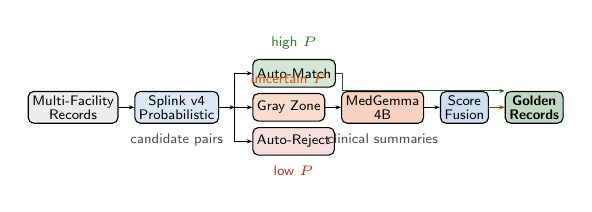
\begin{tikzpicture}[
    node distance=0.2cm and 0.18cm,
    box/.style={draw, rounded corners=2pt, minimum height=0.35cm,
                text centered, font=\fontsize{5}{6}\selectfont\sffamily, inner sep=1.5pt},
    annot/.style={font=\fontsize{4}{5}\selectfont\sffamily, text=black!70},
    arr/.style={-{Stealth[length=2pt]}, thin},
  ]

  % Input
  \node[box, fill=gray!15, align=center] (input) {Multi-Facility\\[-1pt]Records};

  % Splink
  \node[box, fill=tierblue!15, align=center, right=0.2cm of input] (splink) {Splink v4\\[-1pt]Probabilistic};
  \node[annot, below=0.01cm of splink] {candidate pairs};

  % Branch point
  \coordinate[right=0.2cm of splink] (branch);

  % Three tiers
  \node[box, fill=tiergreen!20, above right=0.25cm and 0.22cm of branch] (auto) {Auto-Match};
  \node[annot, above=0.0cm of auto] {\color{tiergreen}high $P$};

  \node[box, fill=tieramber!20, right=0.22cm of branch] (gray) {Gray Zone};
  \node[annot, above=0.0cm of gray] {\color{tieramber}uncertain $P$};

  \node[box, fill=tierred!15, below right=0.25cm and 0.22cm of branch] (reject) {Auto-Reject};
  \node[annot, below=0.0cm of reject] {\color{tierred}low $P$};

  % LLM + Fusion
  \node[box, fill=tieramber!25, align=center, right=0.2cm of gray] (llm) {MedGemma\\[-1pt]4B};
  \node[annot, below=0.01cm of llm] {clinical summaries};

  \node[box, fill=tierblue!20, align=center, right=0.2cm of llm] (fusion) {Score\\[-1pt]Fusion};

  % Golden
  \node[box, fill=tiergreen!30, align=center, right=0.2cm of fusion] (golden) {\textbf{Golden}\\[-1pt]\textbf{Records}};

  % Arrows
  \draw[arr] (input) -- (splink);
  \draw[arr] (splink) -- (branch);
  \draw[arr] (branch) |- (auto);
  \draw[arr] (branch) -- (gray);
  \draw[arr] (branch) |- (reject);
  \draw[arr] (gray) -- (llm);
  \draw[arr] (llm) -- (fusion);
  \draw[arr, tiergreen!70!black] (auto.east) -- ++(0.08,0) |- (golden.north west);
  \draw[arr, tieramber!70!black] (fusion) -- (golden);

\end{tikzpicture}
\caption{ClinFuse three-tier architecture. High-confidence pairs are auto-matched (green) or auto-rejected (red). Only ambiguous gray-zone pairs (amber) are routed through the clinical LLM, keeping compute costs low.}
\label{fig:architecture}
\end{figure}

% =====================================================================
%  3  TECHNICAL DETAILS
% =====================================================================
\section{Technical Details}

\subsection{Data Generation and Augmentation}

Synthea~\cite{walonoski2018} generates realistic synthetic patients with clinically coherent histories spanning conditions, medications, allergies, observations, and procedures. An augmentation pipeline distributes each patient's records across multiple simulated facilities and injects demographic errors: name variations (nickname substitution, typos, maiden name usage), address errors (abbreviation, format variation), date perturbations, identifier errors (SSN transposition, digit substitution), and formatting noise---mirroring documented real-world error patterns~\cite{morris2016}. Separate datasets are generated for training (10{,}000 patients) and evaluation (500 patients, 1{,}275 records across 5 facilities).

\subsection{Adapting MedGemma for Entity Resolution}

\textbf{Text-only adaptation.}
MedGemma~4B is a multimodal model with both vision and text encoders. Since our task is text-only, we strip the vision tower before fine-tuning, reducing from 4.2B to 3.88B parameters while preserving the medical language understanding from pretraining.

\textbf{QLoRA fine-tuning with classification head.}
We apply 4-bit QLoRA~\cite{dettmers2023} (Low-Rank Adaptation~\cite{hu2021lora}) targeting attention and MLP projection layers, and add a binary classification head. Fine-tuned classification heads significantly outperform zero-shot prompting for binary tasks~\cite{finetune_vs_prompt} while being orders of magnitude faster at inference~\cite{cls_head_efficiency}. Training uses balanced match/non-match pairs generated from augmented Synthea records. The fine-tuned adapter and merged model are published on HuggingFace Hub.

\subsection{Results}\label{sec:results}

Table~\ref{tab:results} compares Splink-only matching against the full ClinFuse pipeline on 1{,}275 synthetic records (500 patients across 5 facilities).

\begin{table}[h]
\centering\small
\caption{Entity resolution performance. Splink-only uses the 0.95 auto-match threshold. ClinFuse adds MedGemma gray-zone classification and score fusion.}
\label{tab:results}
\begin{tabular}{@{}lcc@{}}
\toprule
\textbf{Metric} & \textbf{Splink Only} & \textbf{ClinFuse} \\
\midrule
Precision & 1.000 & 0.995 \\
Recall & 0.991 & \textbf{1.000} \\
F1 & 0.995 & \textbf{0.997} \\
\midrule
\multicolumn{3}{@{}l@{}}{\textit{Operational statistics (ClinFuse):}} \\
\multicolumn{2}{@{}l@{}}{~~Gray-zone pairs classified by LLM} & 242 \\
\multicolumn{2}{@{}l@{}}{~~LLM-recovered matches} & 4 \\
\bottomrule
\end{tabular}
\end{table}

At the conservative 0.95 threshold, Splink alone achieves perfect precision but misses true matches in the gray zone. MedGemma's clinical understanding---recognizing matching disease trajectories and overlapping medication regimens---recovers all missed matches, lifting recall from 0.991 to 1.000. The trade-off is a small precision reduction (6 false merges out of 1{,}187 predicted matches)---acceptable given the far higher clinical cost of missed matches. The demographic veto floor prevents the LLM from overriding strong demographic disagreement, keeping false merges rare. The MedGemma classifier achieves 0.93 F1 in standalone evaluation; MedGemma provides clinical understanding that no probabilistic linker can offer, complementing Splink's high-precision demographic matching.

% --- FIGURE 2: Clinical Summary Example ---
\begin{figure}[t]
\centering
\footnotesize
\begin{tabular}{@{}p{0.97\columnwidth}@{}}
\toprule
\textbf{Record A} (Facility 1) \\
\midrule
\texttt{CONDITIONS:} \\
\texttt{~~2018: Hypertension *; Type 2 Diabetes *} \\
\texttt{~~2020: Acute Bronchitis} \\
\texttt{MEDICATIONS:} \\
\texttt{- Metformin 500mg (2018--ongoing)} \\
\texttt{- Lisinopril 10mg (2018--ongoing)} \\
\texttt{OBSERVATIONS:} \\
\texttt{- A1c: 7.2\% (2024-06), 7.0\% (2023-12)} \\
\midrule
\textbf{Record B} (Facility 3) \\
\midrule
\texttt{CONDITIONS:} \\
\texttt{~~2018: Essential Hypertension *; Diabetes *} \\
\texttt{~~2020: Acute Bronchitis} \\
\texttt{MEDICATIONS:} \\
\texttt{- Metformin Hydrochloride 500mg (2018--ongoing)} \\
\texttt{- Lisinopril 10mg (2019--ongoing)} \\
\texttt{OBSERVATIONS:} \\
\texttt{- A1c: 7.2\% (2024-06), 7.0\% (2023-12)} \\
\bottomrule
\end{tabular}
\caption{Structured clinical summary pair as input to the MedGemma classifier. Despite demographic discrepancies (name typo + address abbreviation), the parallel clinical trajectories---identical chronic conditions, overlapping medications, and matching vitals---enable the model to correctly identify a match.}
\label{fig:example}
\end{figure}

\subsection{Deployment and Feasibility}

\textbf{Hardware.} MedGemma 4B runs quantized (4-bit NF4) on a single consumer GPU (e.g., RTX~3090, {\raise.17ex\hbox{$\scriptstyle\sim$}}\$1{,}500). No cloud API dependency.

\textbf{Privacy by design.} All inference is local---no patient data leaves the facility. This satisfies HIPAA and GDPR requirements and supports air-gapped deployment.

\textbf{Cost at scale.} Splink handles {\raise.17ex\hbox{$\scriptstyle\sim$}}95\% of pairs in under 1 second per pair. Only {\raise.17ex\hbox{$\scriptstyle\sim$}}5\% hit the LLM. At hospital scale (100K records), estimated total GPU time is under 1 hour. The pipeline supports both batch processing for MPI deduplication and near-real-time matching for point-of-care patient registration.

\textbf{Integration.} Input is standard HL7/FHIR demographic and clinical fields. Output is a deduplicated Master Patient Index---a drop-in replacement for existing MPI systems. Match and reject thresholds are configurable, allowing operators to tune the precision--recall trade-off for their clinical context.

\textbf{Open source and reproducible.} The complete pipeline is implemented as a DVC directed acyclic graph with separate training and inference tracks. All stages run in Docker containers. Source code, model, adapter, and dataset are publicly available (see Acknowledgments).

\subsection{Limitations and Future Work}

\textbf{Limitations.} ClinFuse is evaluated on synthetic data (Synthea), which, while clinically realistic, may not capture all real-world patterns such as identity theft, deliberate data falsification, or extreme data sparsity in safety-net hospitals. The fusion weights are tuned for this dataset and would require calibration on real EHR data. Synthetic evaluation data may differ in difficulty from real-world data, so reported metrics demonstrate the approach's viability rather than guarantee production performance.

\textbf{Future work.} Key directions include: (1)~validation on de-identified real EHR data to confirm generalization; (2)~\emph{tiered model escalation} where uncertain pairs route from smaller models to larger ones and ultimately to human-in-the-loop review, creating a graduated safety net for the most ambiguous cases; (3)~\emph{multimodal resolution} leveraging MedGemma's vision capabilities to incorporate radiology images and scanned documents as additional identity signals; (4)~joint demographic--clinical fine-tuning in a single end-to-end model; and (5)~embedding-based candidate matching using learned patient representations for fast approximate nearest-neighbor search, replacing handcrafted blocking rules to scale to millions of records.

% =====================================================================
%  CONCLUSION
% =====================================================================
\section{Conclusion}

This work demonstrates that MedGemma---pretrained for clinical QA and medical imaging, never designed for entity resolution---can be effectively repurposed for patient identity matching through QLoRA adaptation. Achieving 0.93 F1 on this novel pairwise classification task, its integration into the ClinFuse pipeline lifts end-to-end recall from 0.991 to a perfect 1.000 while maintaining 99.5\% precision. The system runs entirely on-premises on a single consumer GPU, requires no cloud API, and invokes the LLM only for the small fraction of pairs that probabilistic matching cannot resolve. These properties---high accuracy, full privacy, low cost, and interpretable fusion---make MedGemma-powered entity resolution a practical path toward the 99.9\% matching accuracy that the MATCH~IT Act demands and that patient safety requires.

Entity resolution represents a genuinely novel application of MedGemma---repurposing medical language understanding for a task entirely outside the model's pretraining distribution. The success of this transfer suggests that medical foundation models have broader utility than their original design scope implies: clinical NLP capabilities can power infrastructure tasks that underpin the entire healthcare data ecosystem. As health information exchange scales under TEFCA, MedGemma's combination of clinical reasoning, edge deployability, and adaptability through parameter-efficient fine-tuning offers a foundation for safe, accurate, and privacy-preserving patient matching at national scale.

% =====================================================================
%  ACKNOWLEDGMENTS
% =====================================================================
\section*{Acknowledgments}

This work uses MedGemma~\cite{medgemma} (Google Health AI) as the foundation model and Splink~\cite{splink} for probabilistic linkage. Synthetic data generated with Synthea~\cite{walonoski2018}. Developed for the Kaggle MedGemma Impact Challenge~\cite{kaggle2026}.

\smallskip
\noindent\textbf{Resources:}\\
Code: \url{https://github.com/abicyclerider/clinfuse}\\
Model: \url{https://huggingface.co/abicyclerider/medgemma-4b-entity-resolution-text-only}\\
Dataset: \url{https://huggingface.co/datasets/abicyclerider/entity-resolution-pairs}\\
Video: \textit{[URL TBD before submission]}

% =====================================================================
%  REFERENCES
% =====================================================================
\balance
\begingroup
\small
\begin{thebibliography}{99}

\bibitem{ecri2016}
ECRI Institute PSO, ``Deep dive: Patient identification,'' 2016.

\bibitem{western2026}
J.~Western et al., ``SEE ALTERNATE MRN: Duplicate charts in hospitalized patients,'' \textit{BMJ Qual.\ Saf.}, 2026.

\bibitem{morris2016}
G.~Morris et al., ``Patient matching is a challenge,'' \textit{Perspect.\ HIM}, 2016.

\bibitem{blackbook2018}
Black Book Market Research, ``Provider interoperability and patient record error rates,'' 2018.

\bibitem{onc2014}
ONC, ``Patient identification and matching final report,'' 2014.

\bibitem{harron2019}
K.~Harron et al., ``Linkage error bias,'' \textit{Int.\ J.\ Epidemiol.}, 48(6):2050--2060, 2019.

\bibitem{matchit2025}
U.S.\ Congress, ``MATCH IT Act,'' H.R.~2002, 2025.

\bibitem{tefca2024}
ONC, ``TEFCA v2.1,'' 2024.

\bibitem{fellegi1969}
I.~P. Fellegi and A.~B. Sunter, ``A theory for record linkage,'' \textit{JASA}, 64(328):1183--1210, 1969.

\bibitem{medlink2023}
Z.~Wu et al., ``MedLink: De-identified patient record linkage,'' \textit{Proc.\ KDD}, 2023.

\bibitem{prism2024}
B.~Qian et al., ``PRISM: Patient records interpretation for clinical trial matching using LLMs,'' \textit{npj Digit.\ Med.}, 7, 2024.

\bibitem{medgemma}
Google Health AI, ``MedGemma model card,'' 2025.

\bibitem{splink}
R.~Linacre et al., ``Splink: Probabilistic record linkage at scale,'' \textit{Int.\ J.\ Pop.\ Data Sci.}, 2022.

\bibitem{walonoski2018}
J.~Walonoski et al., ``Synthea: Generating synthetic patients and EHRs,'' \textit{JAMIA}, 25(3):230--238, 2018.

\bibitem{dettmers2023}
T.~Dettmers et al., ``QLoRA: Efficient finetuning of quantized LLMs,'' \textit{NeurIPS}, 2023.

\bibitem{hu2021lora}
E.~J. Hu et al., ``LoRA: Low-rank adaptation of large language models,'' \textit{arXiv:2106.09685}, 2021.

\bibitem{finetune_vs_prompt}
S.~Gao et al., ``Fine-tuned small LLMs vs.\ zero-shot large LLMs for classification,'' \textit{arXiv:2406.08660}, 2024.

\bibitem{cls_head_efficiency}
S.~Singh et al., ``Classification heads: 130x faster than prompting,'' \textit{arXiv:2411.05045}, 2024.

\bibitem{kaggle2026}
F.~Mahvar et al., ``MedGemma Impact Challenge,'' Kaggle, 2026.

\bibitem{peeters2023}
R.~Peeters and C.~Bizer, ``Entity matching using large language models,'' \textit{arXiv:2310.11244}, 2023.

\bibitem{booster2024}
Y.~Li et al., ``On leveraging large language models for enhancing entity resolution: A cost-efficient approach,'' \textit{arXiv:2401.03426}, 2024.

\bibitem{coling2025}
T.~Wang et al., ``Match, compare, or select? An investigation of large language models for entity matching,'' \textit{Proc.\ COLING}, 2025.

\bibitem{pubmedbert_hybrid2025}
C.~Cao et al., ``Linking patient records at scale with a hybrid approach combining contrastive learning and deterministic rules,'' \textit{medRxiv}, 2025.

\end{thebibliography}
\endgroup

\end{document}
